\section{Durchführung}
In der Abbildung (\ref{abb:2}) ist eine schematische Darstellung zur Messung von radioaktiven
Strahlen.
\begin{figure}[H]
  \centering
  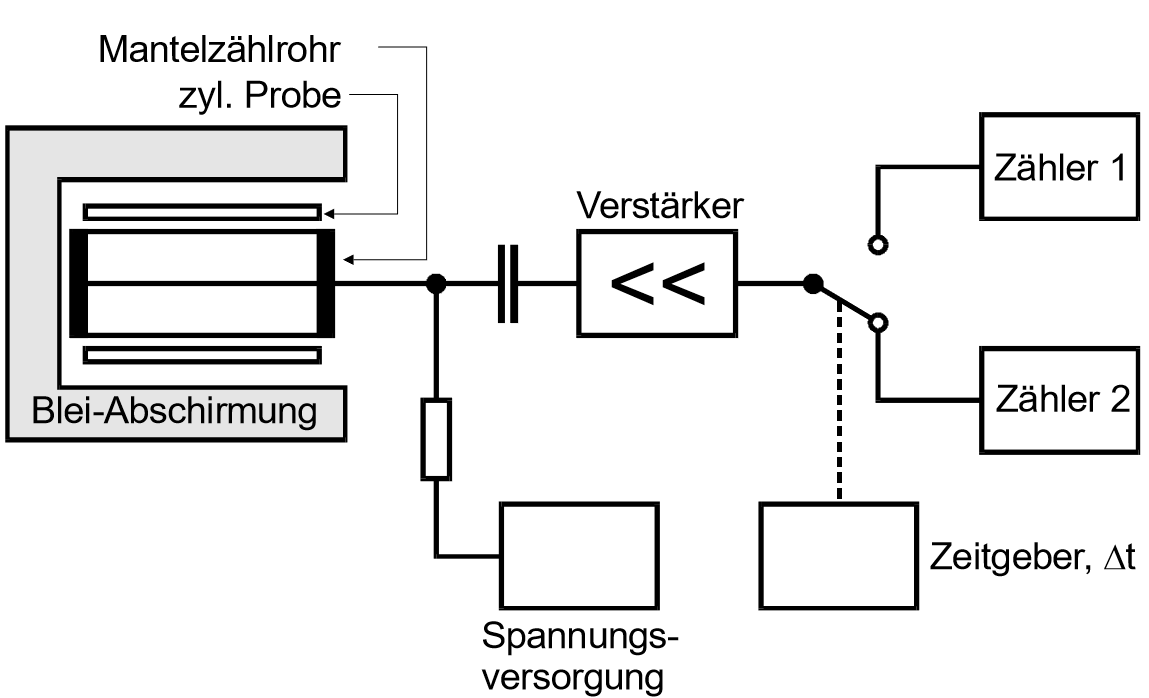
\includegraphics[width=\textwidth]{content/Aufbau.png}
  \caption{Darstellung der Messaperatur \cite{1}.}
\end{figure}
Mit Hilfe einem Geiger-Müller-Zählrohr wird ein konstanter Bruchteil emittierte Strahlung nachgewiesen.
Um mit der Messung anfangen zu können muss zunächst die Messung für den Nulleffekt gestartet werden.
Sie misst kosmische Strahlung sowie die natürliche Radioaktivität und verfälscht möglicherweise die genauen
Messdaten von unseren Proben.
Der Zeitgeber für die Nullmessung wird auf 900 s angesetzt und anschließend wird die Zählrate notiert.
Die erste Probe, ein Silber-Präparat was aus 52,3 \% dem Isotop $\ce{^{107}_{}Ag}$ und zu 48,7 \% dem Isotop $\ce{^{109}_{}Ag}$ besteht, wird eingesetzt.
Der eingestellte Zeitintervall für diese Probe wird
auf 10 s eingestellt und deren Zählrate in jedem Zeitraum notiert.  Die zweite Probe, ein Indium-Präparat was 100 \% aus dem Isotop $\ce{^{103}_{}In}$ besteht,
wird auf den Zeitintervall von 240 s eingestellt und auch hier die Zählrate in jedem Zeitraum notiert.
Die Zeitintervall wurden in einer Tabelle im Labor vorgeschlagen.



\begin{table}
  \centering
  \caption{Messaufnahme von Silber (Ag).}
  \label{tab:1}
  \begin{tabular}{c c c c c c c c}
    \toprule
    $t \, /\, s$& $N_{\Delta t}$& $t \, /\, s$& $N_{\Delta t}$ & $t \, /\, s$& $N_{\Delta t}$ & $t \, /\, s$& $N_{\Delta t}$ \\
    \midrule
    10 & 387 & 130 & 25 & 250 & 10 & 370 & 8\\
    20 & 143 & 140 & 25 & 260 & 14 & 380 & 5\\
    30 & 113 & 150 & 30 & 270 & 20 & 390 & 11\\
    40 & 116 & 160 & 27 & 280 & 13 & 400 & 8\\
    50 & 82 & 170 & 13 & 290 & 10 & 410 & \cellcolor{red}2\\
    60 & 58 & 180 & 27 & 300 & 30 & 420 & 11\\
    70 & 60 & 190 & 18 & 310 & 10 & -&-\\
    80 & 45 & 200 & 21 & 320 & 9 & -& - \\
    90 & 51 & 210 & 17 & 330 & 10 & -&\\
    100 & 36 & 220 & 10 & 340 & 15 &- &-\\
    110 & 33 & 230 & 22 & 350 & 10 &- &-\\
    120 & 31 & 240 & 14 & 360 & 12 &- &-\\
    \bottomrule
  \end{tabular}
\end{table}

\begin{table}
  \centering
  \caption{Messaufnahme von Indium (In).}
  \label{tab:2}
  \begin{tabular}{c c c c}
    \toprule
    $t \, /\, s$& $N_{\Delta t}$& $t \, /\, s$& $N_{\Delta t}$ \\
    \midrule
    240  &  2930 & 2160 & 1773\\
    480  &  2710 & 2400 & 1710\\
    720  &  2604 & 2640 & 1710\\
    960  &  2258 & 2880 & 1543\\
    1200 &  2229 & 3120 & 1514\\
    1440 &  2117 & 3360 & 1446\\
    1680 &  1900 & 3600 & 1436\\
    1920 &  1923 & - & -\\
    \bottomrule
  \end{tabular}
\end{table}
